\subsection{Permitivity depend on frequency}

\begin{frame}{Permitivity depend on frequency}
    \begin{columns}
        \column{0.5\textwidth}
        The polarization:
        \begin{equation*}
            \mathbf{P} = \dfrac{Ne^2}{m} \left( \sum_j \dfrac{f_i}{\omega_j^2 - \omega^2 + i \gamma_j \omega} \right) \mathbf{E}.
        \end{equation*}
        Permitivity:
        \begin{equation*}
            \varepsilon (\omega) = \varepsilon_0\left( 1 + \dfrac{Ne^2}{m \varepsilon_0} \dfrac{f_i}{\omega_0^2 - \omega^2 + i \gamma \omega} \right).
        \end{equation*}
        Anomalous dispersion:
        \begin{equation*}
            n = \sqrt{\varepsilon/\varepsilon_0} \approx 1 + A \left( 1 + \dfrac{B}{\lambda^2} \right).
        \end{equation*}

        \cite{Landau_1984}
        
        \column{0.5\textwidth}
        \vspace{-3mm}
        \begin{figure}
            \centering
            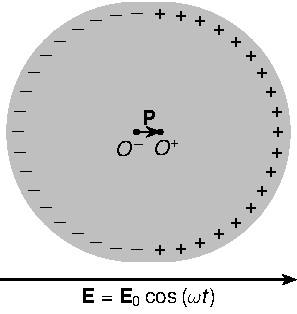
\includegraphics[width=\textwidth]{Figures/Rayleigh_scattering.pdf}
            \caption{Rayleigh scattering.}
            \label{fig:Rayleigh_scattering}
        \end{figure}
    \end{columns}
\end{frame}